\documentclass[aspectratio=169]{beamer}

\usepackage[english]{babel}
\usepackage[utf8x]{inputenc}			
\usepackage{listings}
\usepackage{xcolor}

\lstset{
    language=R,
    basicstyle=\ttfamily\small,
    backgroundcolor=\color{gray!10},
    frame=single,
    breaklines=true,
    showstringspaces=false,
    keywordstyle=\color{blue},
    commentstyle=\color{green!50!black},
    stringstyle=\color{red},
    numbers=none,
    xleftmargin=10pt,
    xrightmargin=10pt,
    framexleftmargin=5pt,
    framexrightmargin=5pt
}

\mode<presentation>						
{
  \usetheme{default}					
  \usecolortheme{default} 			
  \usefonttheme{default}  				
  \setbeamertemplate{caption}[numbered]	
}

\usepackage{graphicx}
\graphicspath{{figure/}}				% Shared figure folder for all labs
\usepackage{booktabs}
\usepackage{hyperref}					
\usepackage{subcaption}  
\usepackage{multicol}
\usepackage{hyperref}

\title{Interval Estimation}	
\author{Rex Shao-Yu Wang}								
\institute{Department of Agronomy, National Taiwan University}				
\date{April 20, 2026}								

\begin{document}

% Title page
\begin{frame}
  \titlepage
\end{frame}

% Outline
\begin{frame}{Outline}
  \tableofcontents
\end{frame}





\section{Sample}
\begin{frame}{Sampling \& Inference}
\begin{figure}
    \centering
    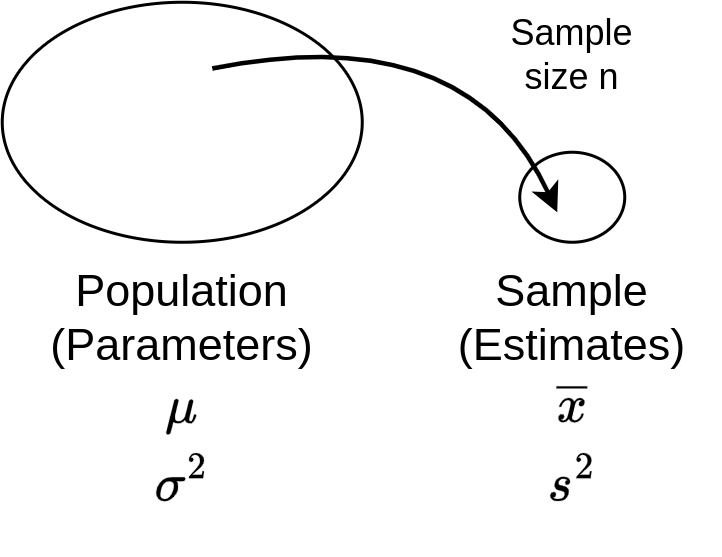
\includegraphics[width=0.5\linewidth]{population_vs_sample.drawio.png}
\end{figure}
\end{frame}




\begin{frame}[fragile]{Sampling}
We can use \texttt{sample(x, size)} function to sample from population.\\
\texttt{size}: The number of sample we want
\begin{lstlisting}
# We randomly generate a vector x
x <- rnorm(10000, 3, 0.5)

# We can use sample() to get a sample from x
sample(x, size = 10)
\end{lstlisting}
\end{frame}




\begin{frame}{Distribution of the Sample Mean}
If we draw a sample of size $n$ from a population where each element follows a normal distribution:
\[
X \sim N(\mu, \sigma^2)
\]

Then the sample mean $\bar{X}$ follows a normal distribution:
\[
\bar{X} \sim N\left(\mu_{\bar{X}} = \mu, \sigma^2_{\bar{X}} = \frac{\sigma^2}{n}\right)
\]
\end{frame}



\begin{frame}{Distribution of mean for various sample sizes}
\begin{figure}
    \centering
    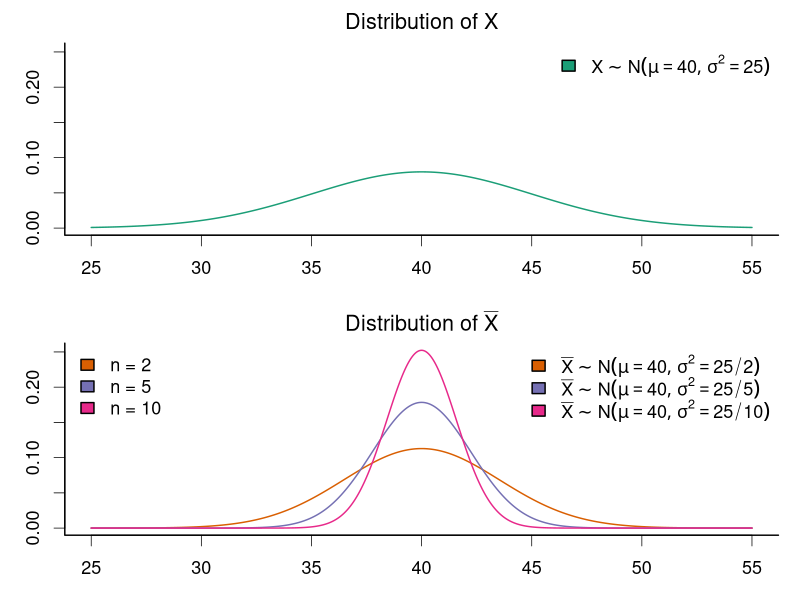
\includegraphics[width=0.7\linewidth]{CI_distribution_xbar.png}
\end{figure}
\end{frame}




\section{Confidence Interval}
\begin{frame}{Confidence Interval ($\sigma^2$ known)}
If population variance $\sigma^2$ is known, then we can build CI for the population mean $\mu$ 
    \begin{align*}
        \overline{X} - Z_{[1-\alpha/2]}\frac{\sigma}{\sqrt{n}}
        \le \mu \le
        \overline{X} + Z_{[1-\alpha/2]}\frac{\sigma}{\sqrt{n}}
    \end{align*}
    \begin{figure}
        \centering
        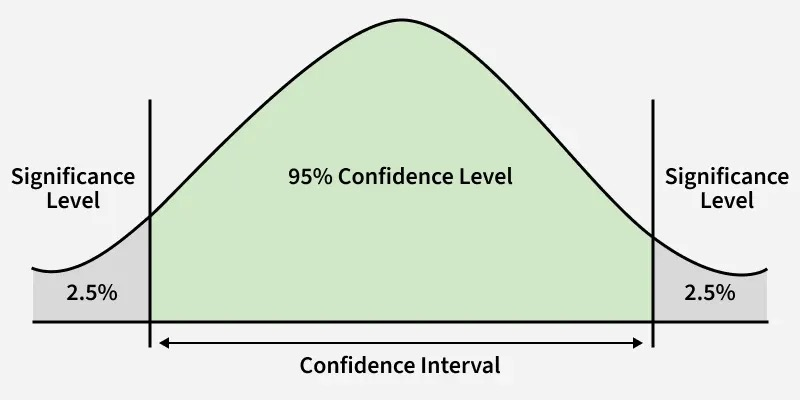
\includegraphics[width=0.6\linewidth]{影像.jpeg}
    \end{figure}
\end{frame}


\begin{frame}[fragile]{Confidence Interval ($\sigma^2$ known)}
Here we’ll use the example mentioned in Steven’s lecture.\\
\begin{itemize}
    \item $X$: Shoulder heights of African elephants
    \item Randomly select 29 elephants $\Rightarrow \ n = 29$ 
    \item Sample mean $\mu_{\overline{x}} = 271$ cm
    \item $\sigma = 20.8\ cm$
\end{itemize}
Calculate the 95\% CI for the true population mean shoulder height for male elephants.
\end{frame}


\begin{frame}[fragile]{Confidence Interval ($\sigma^2$ known)}
First we set the  $\mu_{\overline{x}}$, n, and $\sigma$ that the question gives.
\begin{lstlisting}
mean_value <- 271
n <- 29
standard_deviation <- 20.8
\end{lstlisting}
Then we calculate the standard error $\frac{\sigma}{\sqrt{n}}$
\begin{lstlisting}
standard_error <- standard_deviation / sqrt(n)
\end{lstlisting}
Set the significant level $\alpha$ and calculate Z score. Then get the margin error $Z_{1-\alpha}\frac{\sigma}{\sqrt{n}}$ 
\begin{lstlisting}
alpha <- 0.05
z_score <- qnorm(alpha/2, lower.tail = FALSE) 
margin_error <- z_score * standard_error
\end{lstlisting}
Calculate lower bound = $\overline{X} - Z_{[1-\alpha/2]}\frac{\sigma}{\sqrt{n}}$ and upper bound = $\overline{X} + Z_{[1-\alpha/2]}\frac{\sigma}{\sqrt{n}}$
\begin{lstlisting}
lower_bound <- mean_value - margin_error
upper_bound <- mean_value + margin_error
print(c(lower_bound, upper_bound))
\end{lstlisting}
\end{frame}



\begin{frame}{Confidence Interval ($\sigma^2$ unknown )}
When population variance $\sigma^2$ is unknown, we can construct $100(1 – \alpha)\%$ confidence intervals as before. We shall use $s$ and relevant values from the t distribution instead of using $\alpha$ and the Z distribution
\begin{align*}
    \overline{X} - t_{df, \alpha/2}\frac{s}{\sqrt{n}}
    \le \mu \le
    \overline{X} + t_{df, \alpha/2}\frac{s}{\sqrt{n}}
\end{align*}
    \begin{figure}
        \centering
        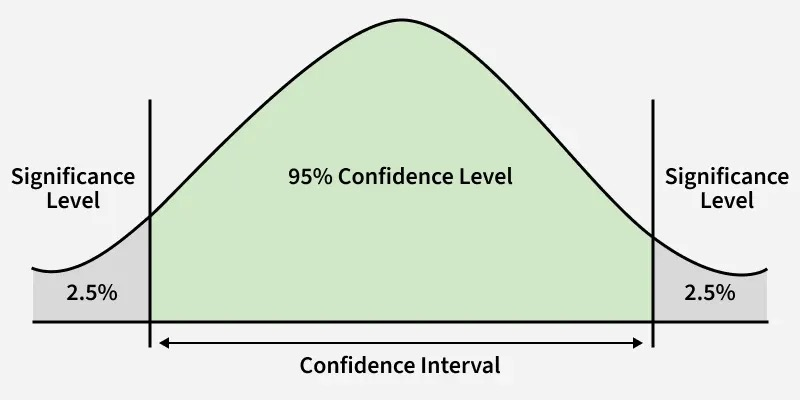
\includegraphics[width=0.6\linewidth]{影像.jpeg}
    \end{figure}
\end{frame}


\begin{frame}[fragile]{Confidence Interval ($\sigma^2$ unknown)}
Here we’ll also use the example mentioned in Steven’s lecture.\\
\begin{itemize}
    \item $X$: Shoulder heights of African elephants
    \item Randomly select 18 elephants $\Rightarrow \ n = 18$ 
    \item Sample mean $\mu_{\overline{x}} = 229$ cm
    \item $s = 15\ cm$
\end{itemize}
Calculate the 95\% confidence interval for the true mean shoulder height for this population of female elephants.
\end{frame}


\begin{frame}[fragile]{Confidence Interval ($\sigma^2$ unknown)}
First we set the  $\mu_{\overline{x}}$, n, and $\sigma$ that the question gives.
\begin{lstlisting}
mean_value <- 229
n <- 18
standard_deviation <- 15
standard_error <- standard_deviation / sqrt(n)
\end{lstlisting}
Set the significant level $\alpha$ and calculate t score. Then get the margin error $t_{df, \alpha}\frac{\sigma}{\sqrt{n}}$ 
\begin{lstlisting}
alpha <- 0.05
degrees_of_freedom <- n - 1
t_score <- qt(alpha, df = degrees_of_freedom, lower.tail = FALSE)
margin_error <- t_score * standard_error
\end{lstlisting}
Calculate lower bound = $\overline{X} - t_{[17, 0.05]}\frac{\sigma}{\sqrt{n}}$ and upper bound = $\overline{X} + t_{[17, 0.05]}\frac{\sigma}{\sqrt{n}}$
\begin{lstlisting}
lower_bound <- mean_value - margin_error
upper_bound <- mean_value + margin_error
print(c(lower_bound, upper_bound))
\end{lstlisting}
\end{frame}


\begin{frame}{Central Limit Theorem (CLT)}
If $X$ is distributed as a random variable (does NOT need to be normal) with  $\mu_{x} =\mu$ and $\sigma^2_{x} = \sigma^2$\\
then  as $n \rightarrow  \infty$
    {\Large
    \begin{gather*}
        \overline{X} \sim N(\mu_{\bar{X}} = \mu, \sigma^2_{\bar{X}} = \sigma^2 / n)
    \end{gather*}
}
We can make inferences about the population mean $\mu$  regardless of the distribution of $X$.\\
As $n$ increase,  $\sigma^2/n$ decreases. $\overline{X}$ is tightly clustered around the population mean $\mu$.\\
\vspace{8pt}
In the following R code, we'll demonstrate how CLT work on certain distribution metioned in the lecture
\end{frame}


\section{Lab Report}
\begin{frame}{Lab Report}
\begin{itemize}
    \item The report file will be in the NTU COOL Assignment section
    \item Submit your file in pdf format
    \item Deadline: 4/26 (Sun) 23:59
    \item Late submission is not accepted
\end{itemize}
\end{frame}
\end{document}




